% !TEX root = ../thesis_main.tex



%%%% --- * --- %%%%
\clearpage	
%\chapter{Estimating Systematic Effects}
\chapter{Analysis and Estimates of Systematic Effects}
\label{systematics_chapter}
\label{analysis_chapter} 
%I really need an excuse to include more pictures of data.  Also, more pictures of simulations.
\missingfigure{Show simulated spectra separated by scattering category.}
\missingfigure{Show SimpleMC spectra, show the supersum, show the superratio, show the superratio asymmetry.  Maybe do some simple fits to show how much better the superratio asymmetry is than \emph{not} the superratio asymmetry.  }


\note[color=jb]{John proposes an intro statement for this chapter (by which I really mean that other chapter, but I'm pretty sure it goes here now).  But anyway, the following two paragraphs are a direct quote from him:  }

%\note[color=jb]{JB:  Here is what I suggest for the intro the Analysis section:  (n.b.:  at the time of this comment, that was Ch.7)
%\\...\\
%7.0
\comment{
Analysis is critical to a precision measurement, as most of the research is in
determining systematic uncertainties by self-consistent analysis and simulations.
Each detector in this experiment is critical and has independent calibrations and cuts.
Full explanation is here (and in two following chapters) justifying choice of the deterministic cuts,
because in the analysis in this thesis the data was not blinded.
The main goal of blinding was nevertheless achieved-- to make sure all analysis is done
completely with full redundancy of checks wherever possible-- so the discipline entailed must
be described in full detail.
Here there are details of detectors:
eMCP
rMCP
beta DSSD
scintillator.
%\\...\\

The collaboration has done an independent analysis fixing bFierz to zero.
Differences with that analysis are interleaved in this section.
Critical physics improvements concern
an emcp-beta timing walk correction which enabled an improved cut against background, also incorporating
a more complete modelling of decay backgrounds from untrapped atoms.
Technical corrections include a correct treatment of the polarization cycle.
An arbitrary change in the deltaE radius cut is kept self-consistent.
}


\note[color=jb]{JB:  ``I doubt I will have further useful comments on the Ch. (((this chapter))) as they are now.}
\note[color=jb]{JB:  \\
I've tried to email you the paragraphs on "collaboration determination of uncertainties" for (((Ch.~\ref{systematics_chapter})))
\\
My intent of all that other advice  was to keep your time spent on Chs 1-4 ((Now Ch. 1-2)) concise, so you could concentrate on these real jobs.  (n.b.:  the advice he's already sent was almost all about chapters 1-4, which are the various intros/background info and experimental setup stuff)
\\ ... \\
I can only say that if you have an equal choice between including a detail or not, pick "not." ''
}

\note[color=jb]{JB:  I will try to schedule meeting with Dan for you to show us the final version of (((Ch.~\ref{systematics_chapter}))) Estimating systematic effects soon.}

%\note[color=org]{Do I want this chapter combined with the analysis chapter?  If that chapter includes all the stuff about G4, it's going to be unwieldy and huge.}
%\note{How do I even \emph{do} these estimations?}

\note[color=todoblue]{JB says:   
\\
A simple estimate from the collaboration that builds intuition for this result:
Scatter in the SiC mirrors and DSSD actually produces an efficiency change at low
beta energy. Energy loss is not minimally ionizing in these structures, and instead
will have a long Landau tail that can take events below energy threshold in the scintillator.
The collaboration has modelled explicitly the false asymmetry as a function
of Kbeta between 600 and 1300 keV, producing roughly (K-0.6 MeV)/(0.7 MeV), i.e.
50\% at Kbeta=0.95 MeV. This efficiency degradation would be distributed roughly equally
between the SiC and DSSD.
If completely ignored, this would introduce by inspection a false bFierz of approximately
0.5.
Scattering effects will vary between linear and sqrt of thickness, so assuming
worst case of linear, the mechanical thickness uncertainty
of 5 micron/300 micron and 6 micron /275 micron, an average of 2\%, making
a random contribution of order 0.01 each.
The Be window has larger mechanical thickness uncertainty of 23micron/229 micron, but
energy loss and scattering in this material is 5x smaller, so the net effect would be similar.
\\ ... \\
To minimize this systematic for future experiments, the collaboration has
implemented pellicle mirrors of negligible thickness, 100 nm Au on 4 micron
kapton. The collaboration is also implementing Be-windowed wire chambers in
place of the DSSD.
\\
...
\\
MJA:  .....huh?
}

\section{Overview}	
A summary of systematics goes here.  In words, yes, but also in table form.


% !TEX root = ../thesis_main.tex



%%%% --- * --- %%%%	
%\renewcommand{\arraystretch}{1.6}

\begin{table}[h!!!!t]
	\begin{center}
	\begin{tabular}{ l  c  c  }
		\multicolumn{1}{l}{ Source} 		& \multicolumn{2}{c}{ \;\;\; \;\;\; Uncertainty \;\;\; \;\;\; }   
		\\
		\multicolumn{1}{l}{ } 				& \multicolumn{1}{c}{\;\; $\bFierz$}   & \multicolumn{1}{c}{$\Abeta$}   	
		\\  \hline
		%%% % %%%
		Scintillator Calibration 			& 0.003								& 0.0003											
		\\
		Scintillator Threshold  			& 0.004 							& 0.0004 						
		\\
		%%% % %%%
		DSSD Individual Strip SNR 			& 0.006								& 0.0007													
		\\
		DSSD Energy Agreement	  			& 0.005 							& 0.0006 						
		\\
		DSSD Detection Radius	  			& 0.006 							& 0.0017 						
		\\
		DSSD Energy Threshold	  			& 0.005 							& 0.0005 						
		\\
		%%% % %%%
		Atomic Cloud			  			& 0.002 							& 0.0002 						
		\\
		%%% % %%%
		Background				  			& 0.004 							& 0.0003 						
		\\
		%%% % %%%
		Beta Scattering				  		& 0.031 							& 0.0025 						
		\\
		%%% % %%%
		Low Energy Tail				  		& 0.008 							& 0.0007 						
		\\
		%%% % %%%
		Mirror Thickness				  	& 0.013 							& 0.0017 						
		\\
		DSSD Thickness				 	 	& 0.013 							& 0.0017 						
		\\
		Beryllium Foil Thickness			& 0.004								& $\!\!\!\!\!\! < 0.0001$ 			
	%	\\
		%%% % %%%
		\\  \hline
		\multicolumn{1}{l}{ Total Systematics} & \multicolumn{1}{c}{0.039}  & \multicolumn{1}{c}{0.0041}
%		Total Systematics			  		& 0.056 							& 0.0055 						
		\\
		\multicolumn{1}{l}{ Statistics} 	   & \multicolumn{1}{c}{0.084}  & \multicolumn{1}{c}{0.0082}
%		Statistics				  			& 0.084 							& 0.0082 						
	%	\\  \hline
		%%% % %%%
	\end{tabular}
	\end{center}
	\caption[Error Budget]{Error budget for the two-parameter analysis for $\bFierz$ and $\Abeta$, with all data included.  All uncertainties are believed to be uncorrelated, and are added in quadrature.  Final results: 
	$\mbox{ $\bFierz = 0.033 \pm 0.084(\textrm{stat}) \pm 0.039(\textrm{sys})$ }$ and $\mbox{ $\Abeta = -0.5738 \pm 0.0082(\textrm{stat}) \pm 0.0041(\textrm{sys})$ }$. }
	\label{table:budget}
\end{table}

%\renewcommand{\arraystretch}{1}




%\label{table:budget}

%	\section{Low-energy Scintillator Threshold}
%	%\\*
	Choice of low-energy scintillator threshold has a large systematic effect...  \aside{It's actually not nearly as big as I'd originally expected.  It's huge in the lineshape thing, but pretty tiny in everything else.}


	\note[color=jb]{from John:  ``I used Ben's threshold when determining the uncertainty from the lineshape tail (UFTLT). 
If you're saying the UFTLT depends on the threshold used, ok, of course it does. But if you're claimiing that UFTLT depends on the **uncertainty** of the threshold, that's manifestly smaller than the UFTLT itself, and I'm going to assert it isn't worth evaluating.''}


\FloatBarrier
\section{Imported Section: ``Comparing Simulations to Experimental Data''}
\label{sec:comparing_data_sims}

\begin{itemize}
	\item Run 3 sets of G4 simulations with a bunch of statistics (N events, for data with like N/10 events).  Each one has the same nominal value of $\Abeta$, but with 3 different values of the scalar coupling $C_S$:  zero, and +/-(whatever).  Keep $C_T=0$.  Because reasons, we're not really able to distinguish between $C_S$ and $C_T$ in this experiment anyway, so might as well keep the analysis simple.
	\item Just run one set of 0.02*N events for the two percent branch.  We can't neglect it, but it isn't going to change much when we adjust BSM couplings.  Just use the old event generator from Holstein Eq.~(51).
	\item Match cuts in simulated data up to the cuts on experimental data.  Obviously.  DSSD cut, DSSD energy, one hit DSSD, one hit scint.  TOF cut, which requires a whole extra model of background in the TOF spectrum (see Section~\ref{sec:tof_bg}).
	\begin{itemize}
		\item Suppose background in the TOF spectrum is coming from decays of atoms that have gotten themselves stuck to surfaces within the chamber...
		\item Run G4 to get a beta TOF spectrum (w.r.t. the decay)
		\item Run COMSOL (credit to Alexandre) to track low-energy SOEs through the electric field from wherever they started, into the detectors.  Energy spectra from Levinger.
		\item Combine G4 and COMSOL spectra, event-by-event, while requiring that both the beta detector and the eMCP are hit according to the set of random numbers generated by each monte carlo separately.  Then, the beta and SOE will each have a TOF from decay to detector, and subtracting one from the other gives a timing spectrum that can be observed experimentally.  See Fig.~\ref{fig:soetof}.
		\item Upper limit for the fraction of events generated this way can be estimated by assuming that all losses from the trap not due to radioactive decay emerge isotropically from the trap and then stick to whatever chamber wall is in its path.  This upper limit is too big by a factor of 2.
	\end{itemize}
	\item For each of those 3 simulations, sort the ``good'' data according to emission angle relative to the detector.  Do each detector individually.  For both polarizations.
	\item Assemble the (simulated) superratio asymmetry.  We'll compare it to data, and the $\chi^2$ from that comparison will be our figure of merit.  
	\item We can make a whole 2D parameter space for different values of $\Abeta$ and $\bFierz$, and compare them all (via their superratio asymmetries) to the experimental data.  We get the ``best'' values of $\Abeta$ and $\bFierz$, where $\chi^2$ is minimized.
	\item We can do this whole thing again for simulated data sets with different values of parameters that we vary as systematics.  Note how the best values of $\Abeta$ and $\bFierz$ change when each of the systematics are varied.
\end{itemize}



\FloatBarrier
\section{BB1 Radius, Energy Threshold, Agreement}
\label{section:bb1_systematics}
	%\\*
BB1 radius cut can help to eliminate scattered events.  Energy threshold selection and statistical agreement between BB1 detectors' energies only makes a small effect on results.  BB1 radius itself has a pretty big effect on the result, but we can at least just G4 it away.  The remaining systematic effect is pretty small.  
\note[color=jb]{JB:  I hope the discussion is clear in your head.  Any effect that relies on scattering computation in G4 should have an uncertainty on order 10\% of the correction -- hopefully you are keeping a distinction here between the finite geometry acceptance (which I guess is exact) scattering off the collimator.}
\note[color=jb]{As per JB's comment in section~\ref{thesisconventionjb}:   ``statistical agreement between BB1 X and Y detectors' energies only makes a small effect on results" does not need the technical details beyond that statement."}
	
\missingfigure{Surely this requires at *least* one image of the pixelated BB1 data.  Maybe some of a few waveforms and energy distributions too.  ....Feels like cheating to include some of that stuff, since Ben was the one who actually used it mostly.}
\note[color=jb]{JB on missing figure:  ``if you used such an image as part of your uncertainty estimate, yes [include it]''}

\note{Remember:  There's noise applied to simulated BB1s, matching some spectrum.}
In the end, we get our results from the scintillator energy only, without summing the BB1 energy back in.  Energy absorbed in DSSDs is only used as (a) a tag for events, and (b) contributing to the total beta energy loss before the beta arrives at the scintillator.
\note[color=jb]{JB:  The simulations of course include it event-by-event, not just a minimally ionizing average loss.}




%
\section{Background Modeling -- Decay from Surfaces within the Chamber}
\note[color=org]{This content got moved to Ch.~\ref{sec:tof_bg}.}
%%%	So many surfaces, all of which can get stray 37K atoms stuck to them.  Then they decay from a place that isn't the actual trap center, and it contaminates our stuff.
%%%	
%%%%	\missingfigure{Show modelled TOF spectra in comparison with real TOF spectra.  Show the cut we made on that. }
%%%	\note[color=jb]{JB on figures that might go here:  Figure 6.4 (currently that picture of the TOF spectrum) could either be here, or you could reference it from here. The TOF histogram is a great start. Adding the asymmetry[TOF] indeed would be vital.}
%%%	\missingfigure{Show the "average asymmetry" (all energies) as a function of TOF, with real data, best model normalization, and extrema of model normalizations.  Show our cut.  Turns out, it's a lot of work for a really tiny correction.  Oh well.}
%%%	\note[color=jb]{JB on the *actual* figure I had been planning to put here, and my remarks about it:  Indeed it will be critical to show a clear compelling version of this figure in thesis and in a paper.  It was vital to minimize and determine this background to avoid fitting a polynomial to it from the wings,  even more so for the energy dependence of A than for its average -- you should say so.
%%%	\\ ... \\
%%%The reason the correction is small is because of all your hard work.}
%%%	
%%%	We model the beta TOF from the surfaces in G4, event by event.  This is necessary because scattered \aside[color=jb]{JB:  ``I wouldn't call these "scattered" events... that's very misleading.'' 
%%%	\\ ... \\ 
%%%	Yeah, I should really stop doing that.  
%%%	\\ ... \\ 
%%%	Wait no, scattered is what I mean!  But fine, my phrasing is really unclear.} events will have their TOF changed to account for a longer beta pathlength, and we're preferrentially cutting away the events that don't have a TOF in the appropriate range.  ....And then have COMSOL generate electron TOFs for SOEs starting from the start points picked by G4.  Ran COMSOL for 0 eV SOEs, and again for Levinger spectrum SOEs.  Used ~9\% 0eV SOEs in the end.  I forget which Levinger distribution I used in the end.  \aside[color=jb]{JB:  Please comment on whether or not it was important to have this energy distribution.}  The point is, for each event, you've simulated a beta TOF that may or may not be scattered off of something before it hits a detector, and you have a SOE TOF for an event originating at that same point, so you subtract them to model the TOF you'd measure in an experiment.  Also, because you've done the scattering with G4, you get the beta energy corrected for any scattering that happened.  This way, one can estimate %\aside[color=jb]{JB:  `you know precisely' $\rightarrow$ `you can estimate'} 
%%%how many ``bad" events are eliminated with the TOF cut, as well as the fraction of ``bad'' events left in what remains.
%%%	
%%%%	\subsection{Decay from Chamber Surfaces}

%
\section{Quantifying the Effects of Backscatter with Geant4}
\note[color=org]{This content got moved over *there*.  (ie, Section~\ref{sec:bs}.)}

%%%% --- * --- %%%%
\section{Lineshape Reconstruction}
\label{sec:lineshape_results}
	\note[color=org]{A lot of this content has gone into (Section~\ref{sec:responsefunction}) instead.  I really need to just mention it here (Sec.~\ref{sec:lineshape_results}) and give an indication of how good the result is.  Then evaluate stuff.}
%	\note[color=jb]{This section should reference Clifford.~\cite{clifford}.}
	Clifford tells us what to do.~\cite{clifford}.
%	\subsection{Motivation}
%	This process is used because the (back-)scatter, which it itself an important systematic, is largely independent of a wide variety of other experimental effects.  These other effects must all be evaluated, but it is computationally prohibitive to re-evaluate the scattering with every other effect under consideration.
	
	\subsection{What is it and how does it work?}
	Mono-energetic beta decay events are generated in GEANT4, which outputs an energy spectrum for unscattered and forward-scattered beta events in the detector.  These spectra are fit to a function to model the scintillator resolution, as well as energy loss in materials that the beta passed through before arriving at the scintillator.  These spectrum fits are performed for a set of beta energies, and parameters are extrapolated to be applied to betas emitted at intermediate energies.  Thus, the whole spectrum can be modeled.  Pictures will make this clearer. 
	
    \begin{figure}[h!!!t]
    	\centering
    	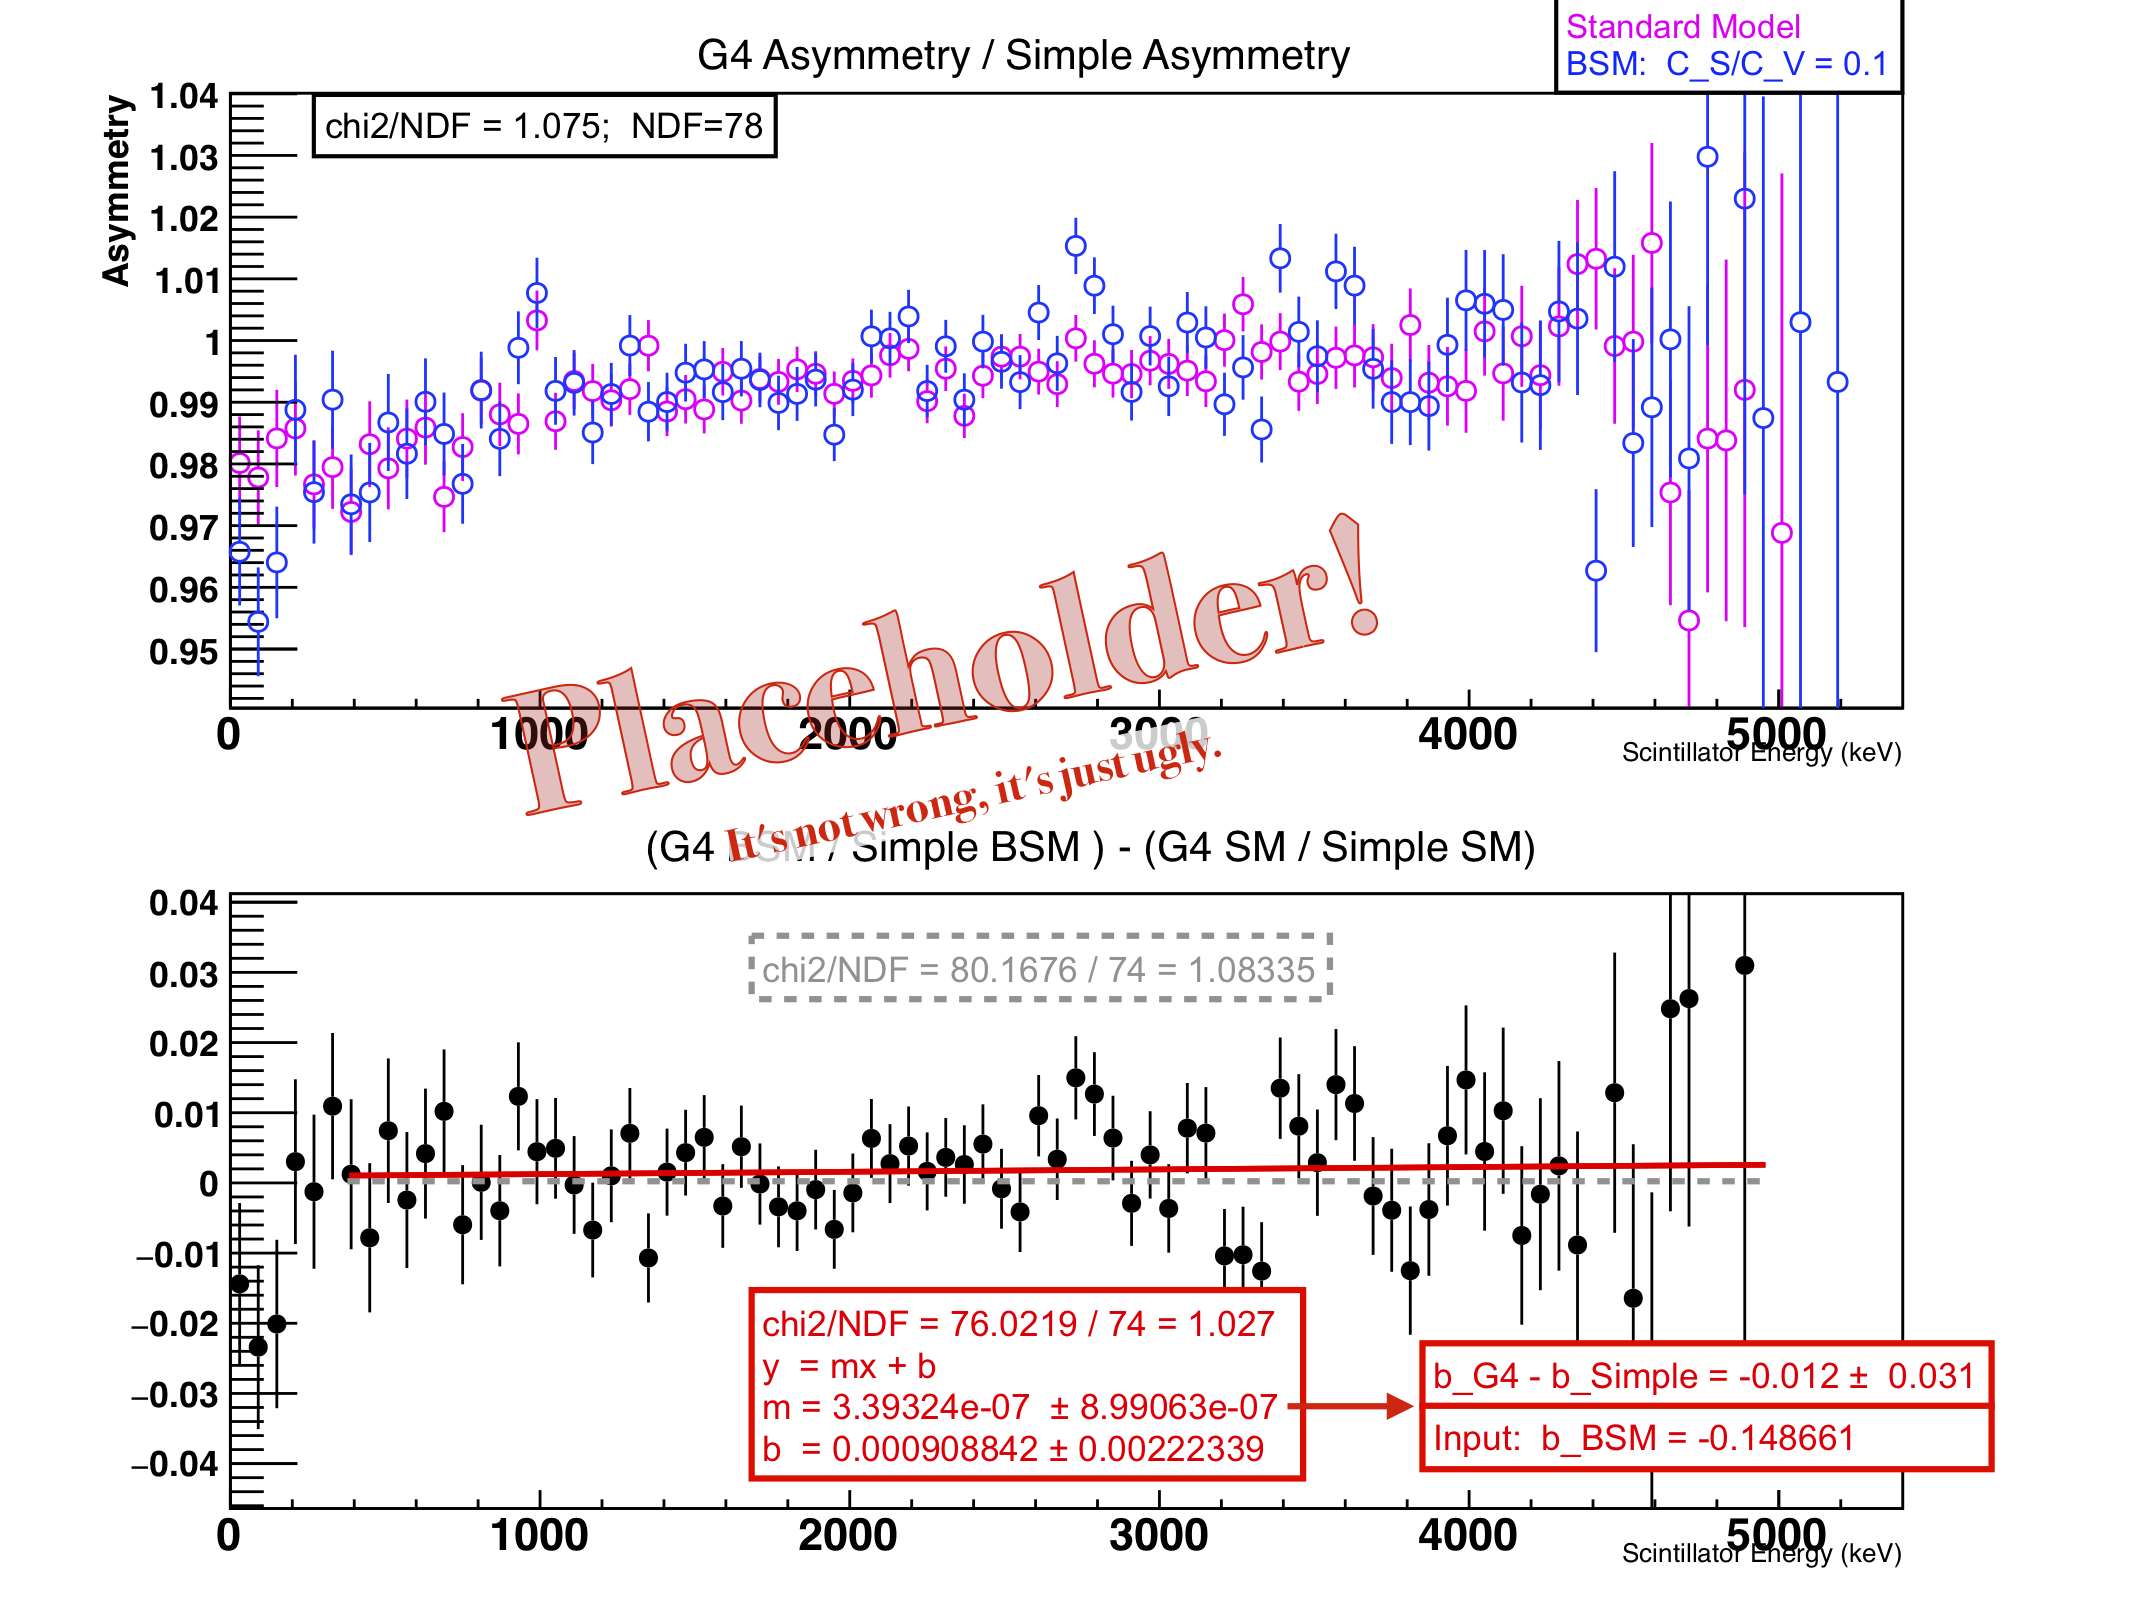
\includegraphics[width=.999\linewidth]
    	{Figures/LineshapeDemo_prelim.png}
    	\caption[Lineshape Comparison]{I'm not actually sure if this picture shows what I want it to.  The point is, if I apply this rough lineshape to stuff that I SimpleMC-ed, then I can evaluate that way various systematic effects that would be time-consuming to actually simulate with G4.  This picture is  *supposed* to be a demonstration that this approach actually works... }    	\label{fig:lineshape_demo}
    \end{figure}
	
%	\subsection{The Math-Specifics}
%	I'll write down the specific functions I'm using, and the parameter values I'm using.  (Maybe this should go in an appendix instead?)  I'll describe the adjustments I make to the spectrum so that it can work even for the dataset where the scintillators' resolutions have changed.
	
	\subsection{The Results -- Things That Got Evaluated This Way}
	As it turns out, only cloud parameters were evaluated this way. \aside[color=jb]{JB:  so it's still critical to write down more of the lineshape work.}
Trap position, size, sail velocity, temperature.  But then we varied the lineshape anyhow, to account for G4 doing a bad job of modelling the bremsstrahlung (sp?).
	%Thicknesses of the SiC mirror, the Be foil, and the DSSD.  Scintillator calibration.  
	\note[color=jb]{JB:  yes, brems strahlung is 'braking radiation' so gets 2 ss's. 
the lineshape tail in any scintillator also includes backscattered events -- we are not claiming the 2-pixel cut is complete}
	
	    \begin{figure}[h!!]
    	\centering
    	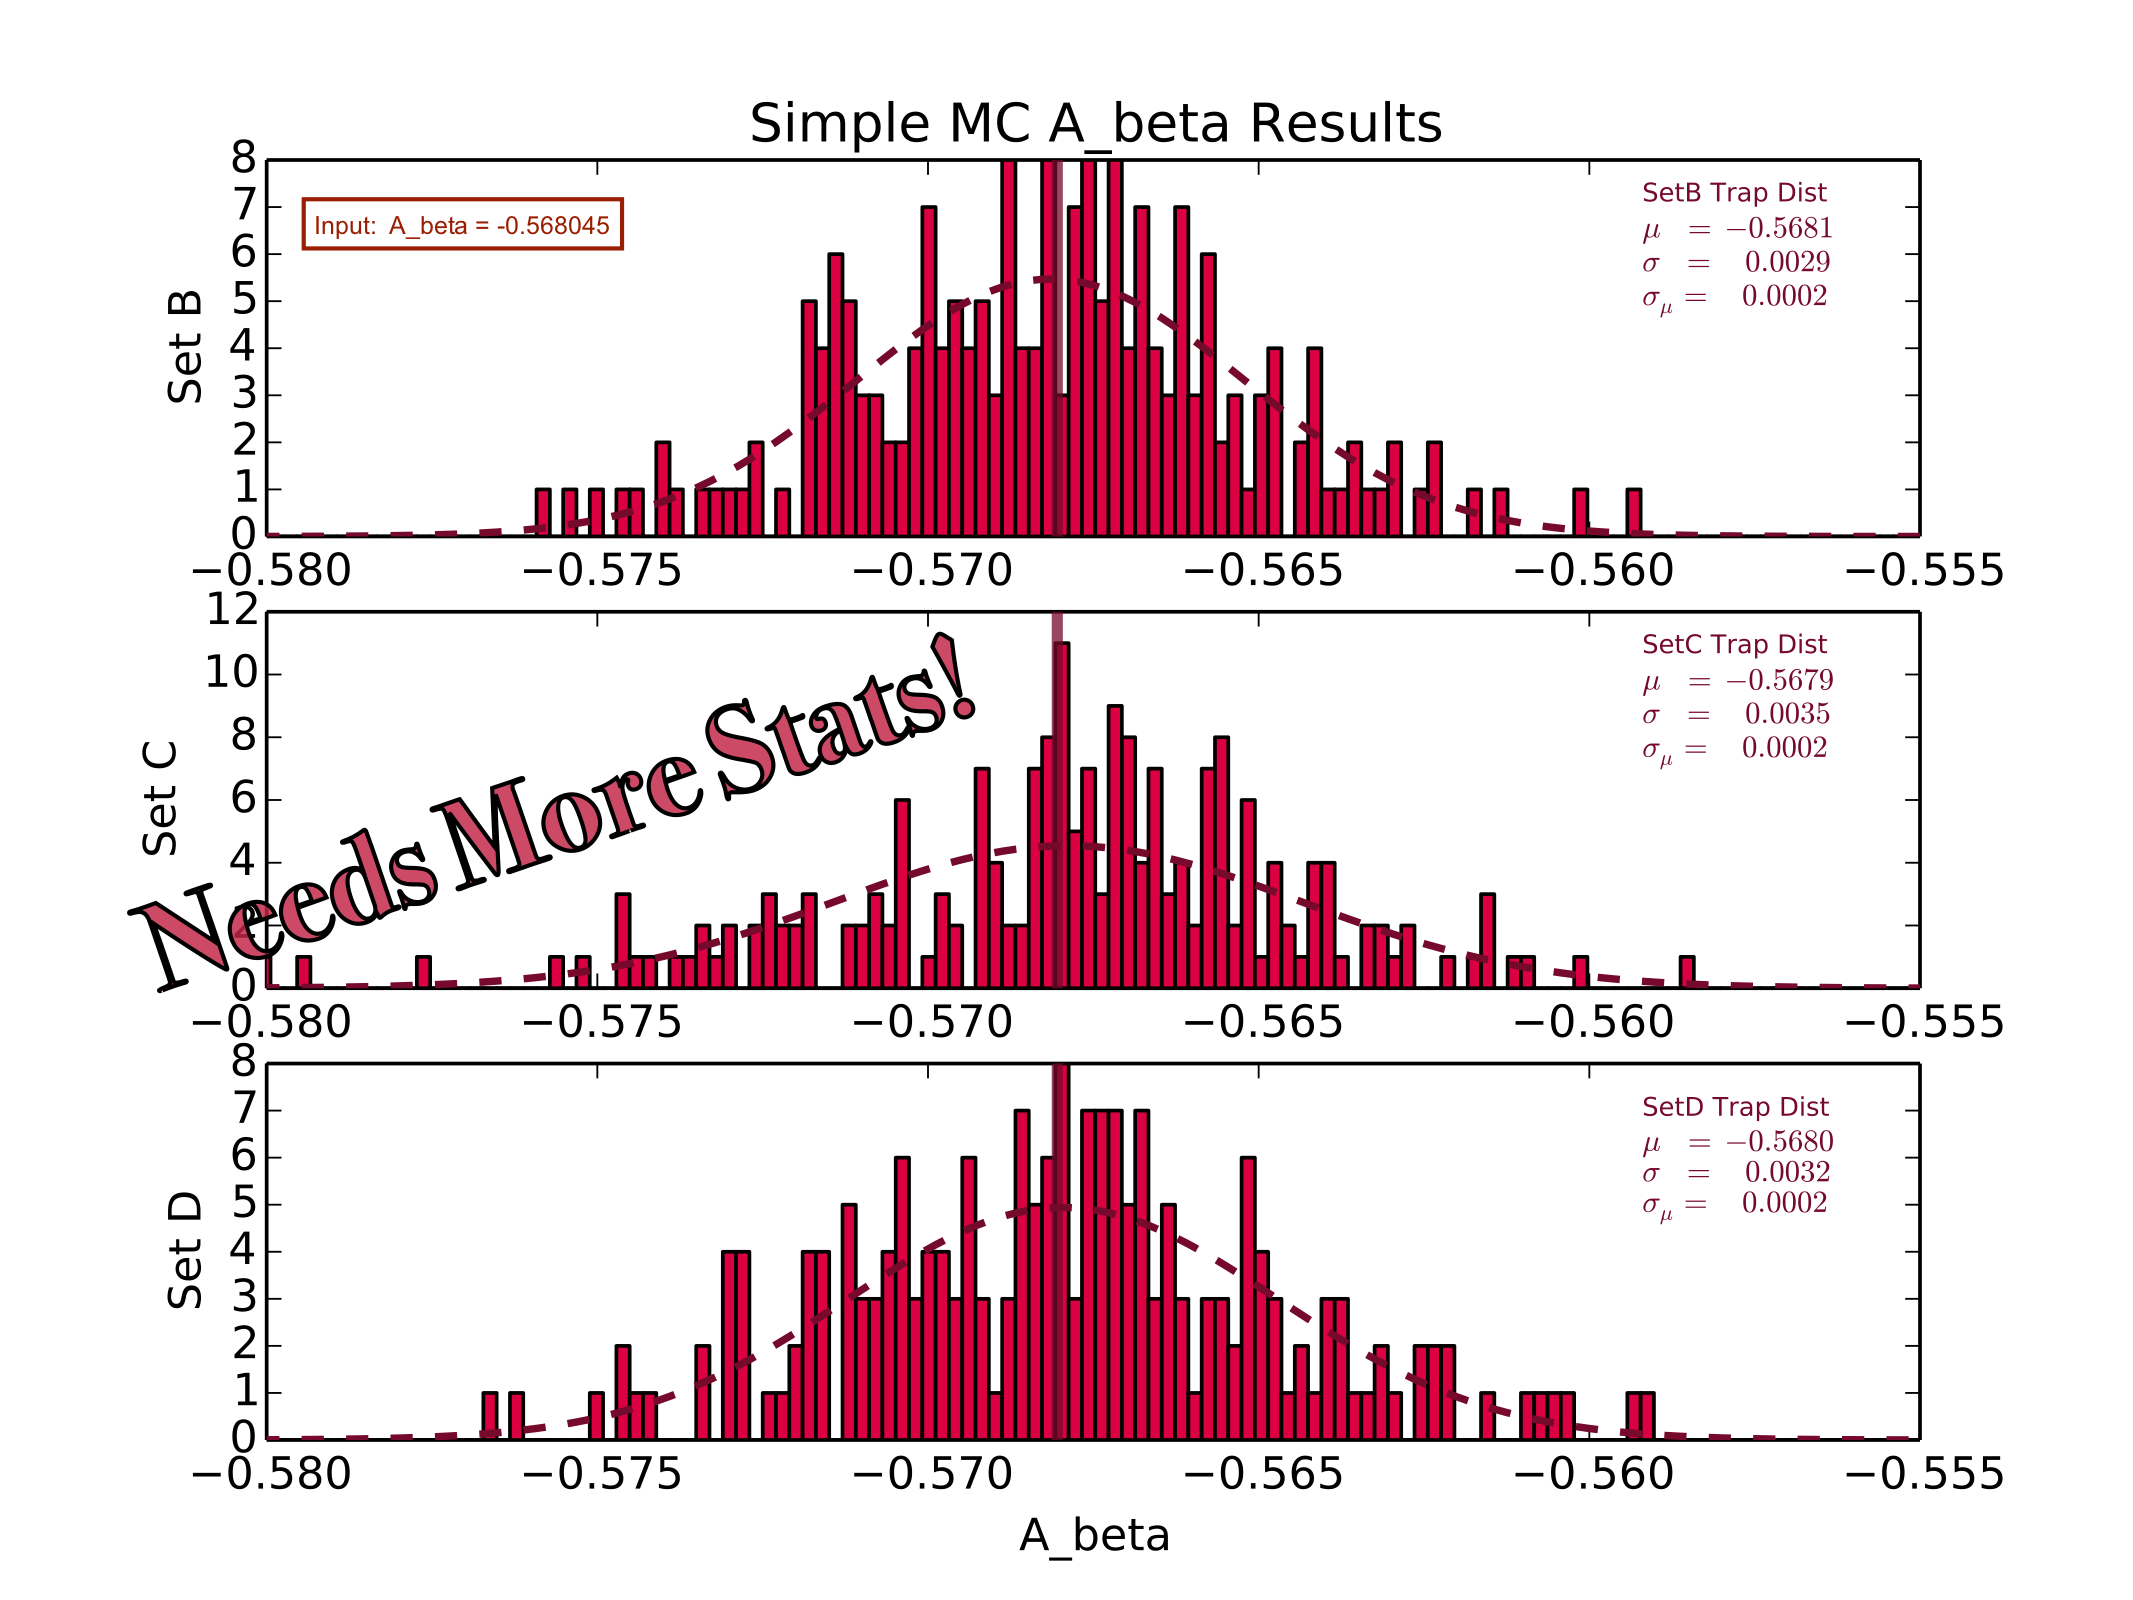
\includegraphics[width=.999\linewidth]
    	{Figures/Position_Err_Abeta_prelim.png}
    	\caption[$\Abeta$ Position Error]{Estimated uncertainty in $\Abeta$ resulting from uncertainty and variation in the cloud parameters.  Evaluated by the lineshape reconstruction method.}	
    	\label{fig:Abeta_position_err}
		\end{figure}

	    \begin{figure}[h!!]
    	\centering
    	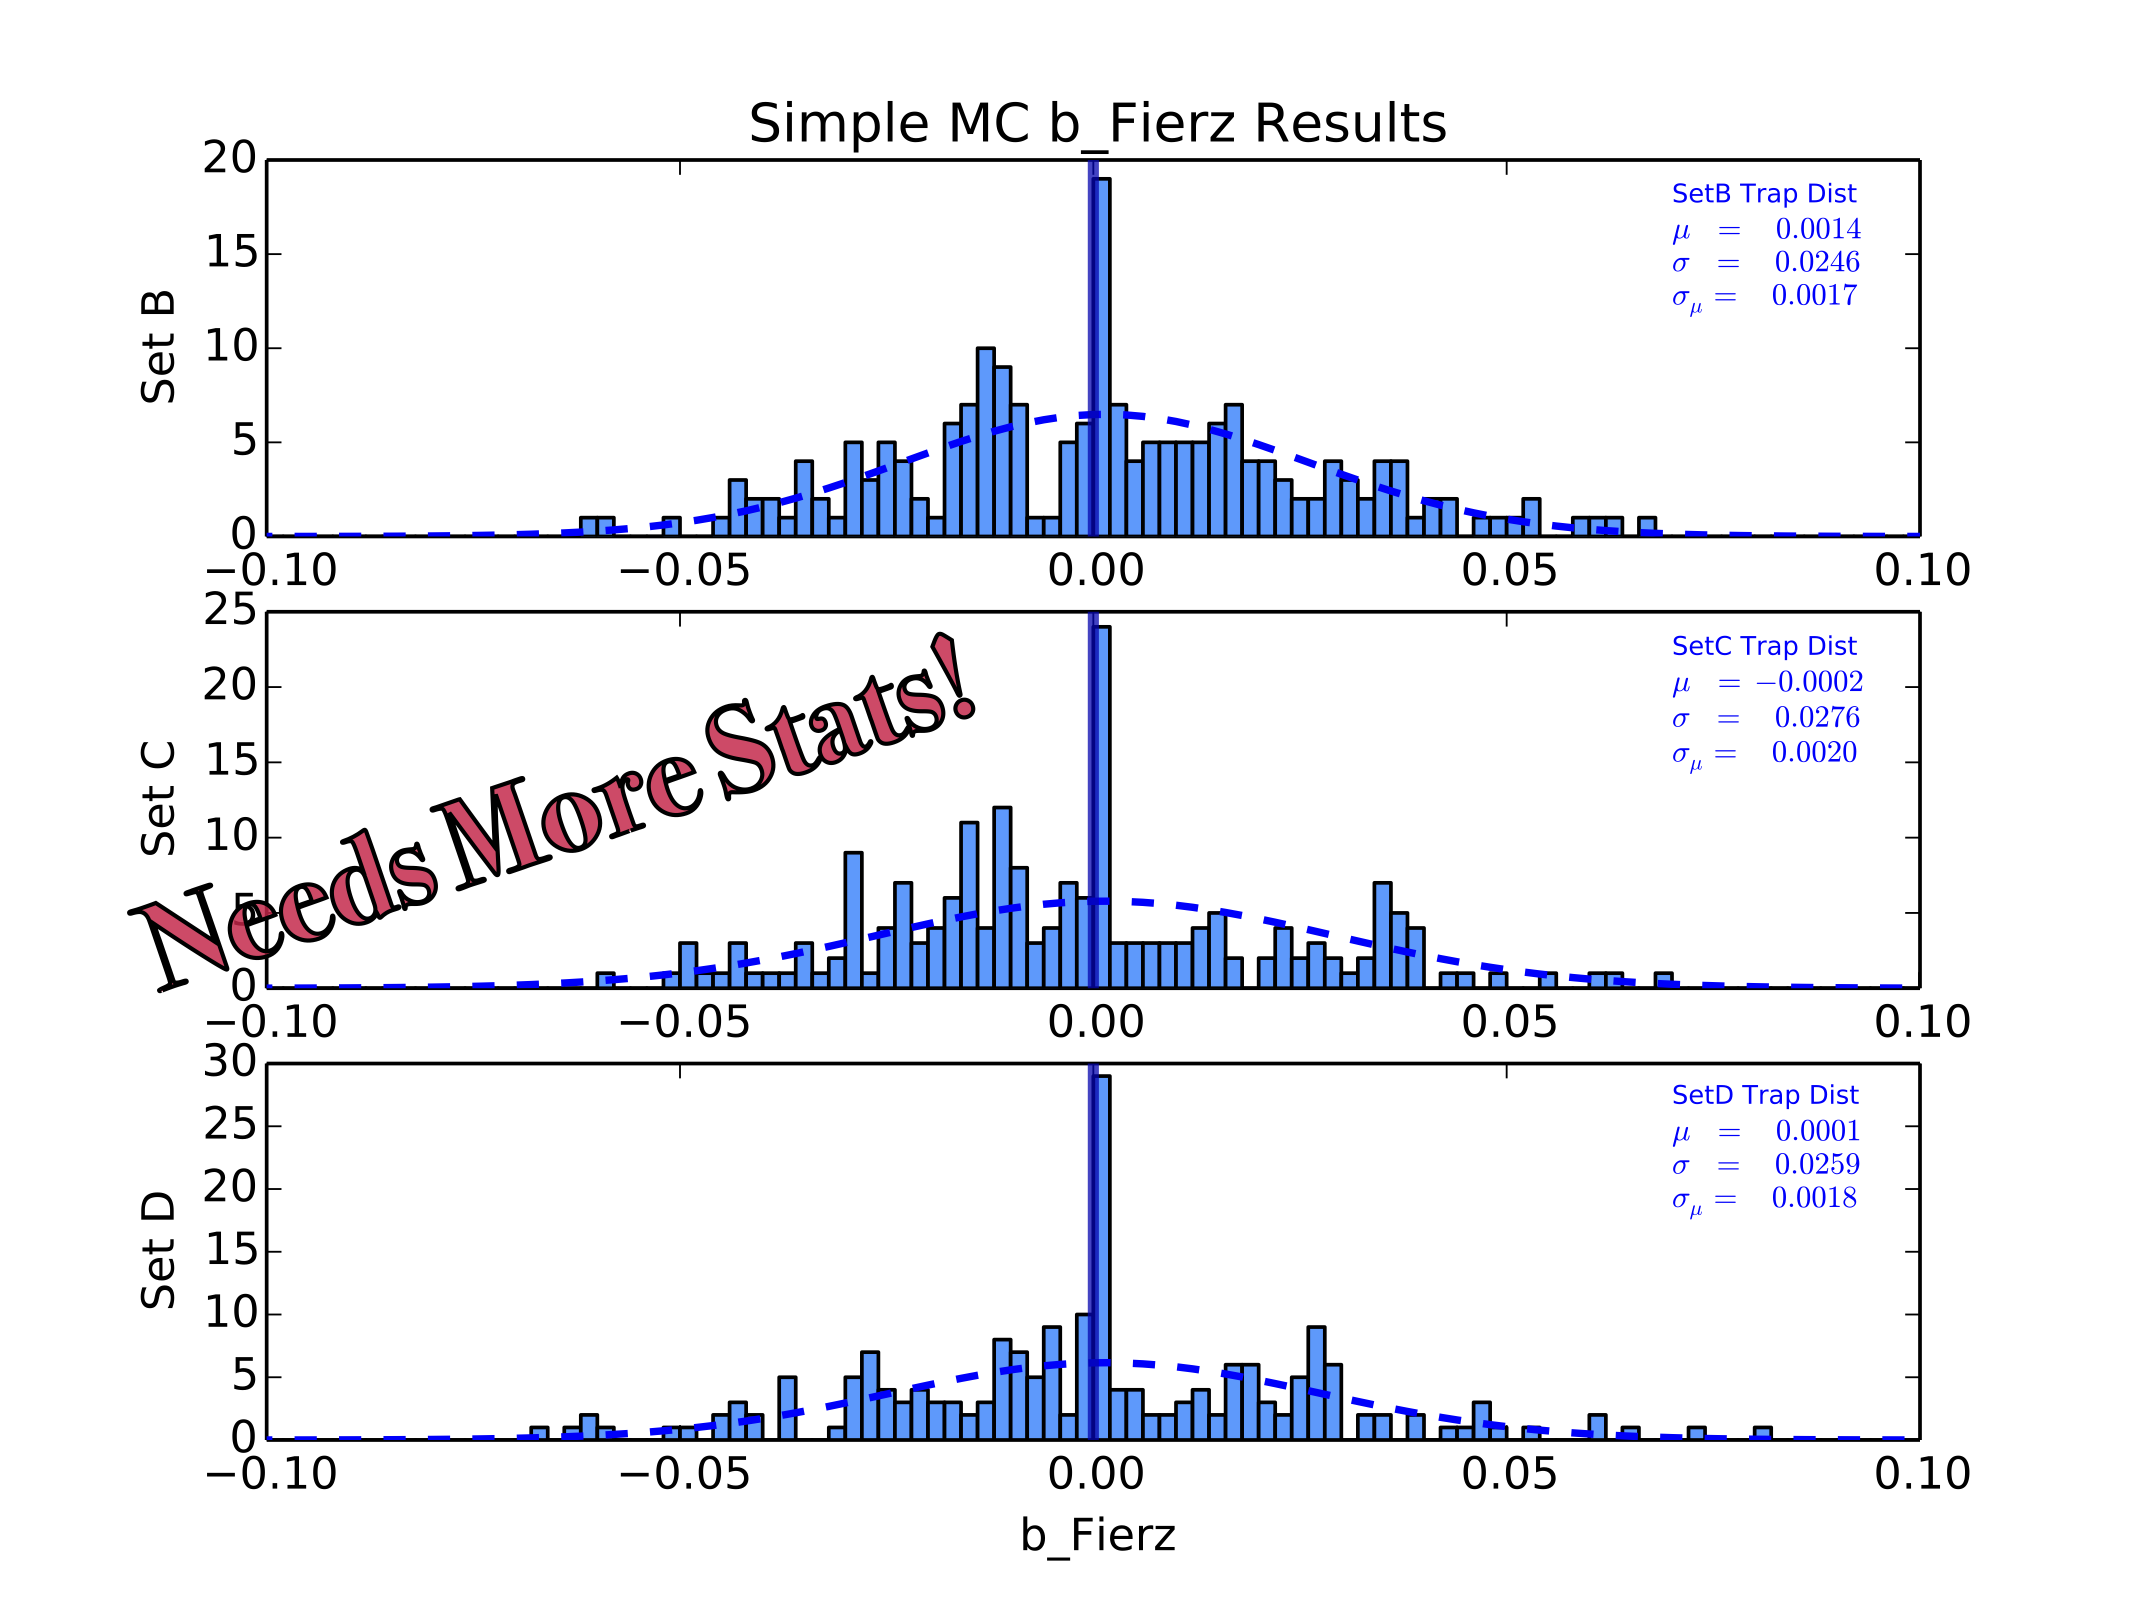
\includegraphics[width=.999\linewidth]
    	{Figures/Position_Err_bFierz_prelim.png}
    	\caption[$\bFierz$ Position Error]{Estimated uncertainty in $\bFierz$ resulting from uncertainty and variation in the cloud parameters.  Evaluated by the lineshape reconstruction method.}		
    	\label{fig:bFierz_position_err}
		\end{figure}

	
	\subsection{The low-energy tail uncertainty, and what it does}
	Bremsstrahlung.  It does Bremsstrahlung.
%	\note[color=jb]{JB:  ``I will write this up better soon."  (I think he already did that)}
\note[color=jb]{ Here is Subsection 9.5.5 ``The low-energy tail uncerainty, and what it does'' complete.  There should be no figure.
\\
Direct quote from John follows in the next two paragraphs.  Maybe I should paraphrase, but it's so nicely written! }

\comment{
This subsection has the collaboration's evaluation of the uncertainty from
the scintillator detector's lineshape tail.
The energy from a monoenergetic beta is not always fully absorbed
in a plastic scintillator.
Although most backscattered betas are vetoed by the DSSD,
some produce bremsstrahlung photons,
and these frequently escape low-Z plastic scintillator-- all cross-sections
are known to high accuracy, but there is always uncertainty entailed in  the
MC implementation.
This lineshape tail will then effectively move events from higher to lower measured
energy, artificially altering the lower-energy asymmetries and mimicking the effects of a
Fierz term.

Since this detector effect is difficult to disentangle from the other scattering
effects off volumes,
the collaboration adds a linear function down to zero for the tail to
a Gaussian for the peak,
with linewidth varying by photon statistics~\cite{clifford}.
The convolution of this simple detector response function with v/c then scales the
centroid MC, with the lineshape tail varied by $\pm$10\% of its value,
a generic uncertainty accepted by the community for MC electromagnetic simulations.
The fit $b_{\rm Fierz}$ centroid changes by $\pm$ 0.0076, summarized
as the 0.008 ``Low Energy Tail'' in the systematics table at the start of this chapter.
Compared to other uncertainties of the present data set,
this is small enough that the accuracy of this estimate is adequate.
}

%\note[color=jb]{End direct quote paragraphs from John.}

%\section{Summary of Data Collected}
%\missingfigure{TBH, the thing that's missing is a table, not a figure.  Needs a table full of systematic errors.  And maybe statistical errors?  wev.}
%\note{Needs an error budget table.  Because of course it fucking does.}

